\documentclass[11pt,class=report,crop=false]{standalone}
\usepackage[screen]{../mathgame}



\begin{document}

\newcommand{\Cl}{\operatorname{\it Cl}}

%====================================================================
\chapitre{Lancer de rayons II}
%====================================================================

%
%\insertvideo{yUgpElITYTg}{partie 5.1. Bits classiques}
%
%\insertvideo{iET0snUXj0k}{partie 5.2. Portes logiques}
%
%\insertvideo{JKmC2u5kvKg}{partie 5.3. Algorithme et complexité}



\objectifs{Nous expliquons en détail la technique du ray-tracing et présentons des outils pour accélérer cette méthode.}

\index{ray tracing@\emph{ray tracing}}

%%%%%%%%%%%%%%%%%%%%%%%%%%%%%%%%%%%%%%%%%%%%%%%%%%%%%%%%%%%%%%%%%%%%%
\section{Les ancêtres du lancer de rayons}

Nous allons voir deux algorithmes qui permettent de transformer une scène en une image comme si on voyait les objets du dessus et d'assez loin.

%--------------------------------------------------------------------
\subsection{Algorithme du $z$-buffer}

\index{algorithme!du z-buffer}

Il s'agit en quelque sorte de lancer des rayons parallèles à l'axe $(Oz)$ et, pour chaque pixel, de calculer quel est l'objet le plus proche.

\myfigure{0.9}{
	\tikzinput{fig-rayonsbis-ancetre-01}
}  

Nous avons des \emph{objets} $\mathcal{O}_k$, chaque objet est un ensemble de $(i,j,z,\Cl)$ où $z$ est la profondeur associée au pixel $(i,j)$ et $\Cl$ est sa couleur ($z$ et $\Cl$ dépendent de $(i,j)$).
(Sur le dessin ci-dessus les objets de la scène sont en 2D mais pourraient aussi être en 3D.)
L'\emph{écran} ou l'\emph{image} est un ensemble de $(i,j,\Cl)$ où $\Cl$ représente la couleur du pixel $(i,j)$. D'un point de vue matériel c'est une zone de la mémoire graphique (\emph{buffer}). On initialise la couleur de tous les pixels à la couleur de fond (par exemple blanc ou transparent).

On a besoin en plus d'un $z$-\emph{buffer} composé de $(i,j,z)$ qui à la fin stocke la profondeur $z$ de l'objet le plus proche pour les coordonnées $(i,j)$.
On initialisera toutes les profondeurs à $+\infty$.

\begin{algorithme}[Algorithme du $z$-buffer]
Pour chaque $(i,j)$ :
\begin{itemize}
	\item Initialiser \ci{prof} à $+\infty$.
	
	\item Pour chaque objet $\mathcal{O}_k$ :
	\begin{itemize}
		\item si $(i,j,z,\Cl)$ vérifie $z < $ \ci{prof} :
		\begin{itemize}
			\item colorer le pixel $(i,j)$ de l'écran avec la couleur $\Cl$,
			\item faire \ci{prof} $\leftarrow z$.
		\end{itemize}
	\end{itemize}
\end{itemize}
\end{algorithme}


\myfigure{0.9}{
	\tikzinput{fig-rayonsbis-ancetre-02}
}  

L'algorithme a le mérite de la simplicité, chaque pixel se voit attribuer la couleur de l'objet le plus proche. Il fonctionne même avec des objets entrelacés.
La position des objets de la scène est rendue fidèlement du point de vue de l'observateur mais l'affichage ne tient pas compte de l'éclairage.


\myfigure{0.4}{
	\tikzinput{anneaux}
} 

%--------------------------------------------------------------------
\subsection{Algorithme du peintre ($z$-\emph{sorting})}

\index{algorithme!du peintre}

Son nom vient de l'analogie avec un peintre qui part d'une toile blanche puis applique de la peinture en plusieurs touches et retouches ; à la fin seules sont visibles les couleurs de la couche supérieure.
La démarche est semblable à la méthode précédente, mais ici on suppose que les objets ne s'entrelacent pas dans la profondeur.


La première partie de l'algorithme consiste à ordonner les objets du plus loin ($z$ grand) au plus proche ($z$ petit).

\myfigure{0.9}{
	\tikzinput{fig-rayonsbis-ancetre-03}
} 

On dessine les objets un par un à l'écran (autrement dit on met à jour la partie de la mémoire de l'écran correspondant aux pixels de l'objet) en partant du plus éloigné et en terminant par le plus proche.

\myfigure{0.7}{
	\tikzinput{fig-rayonsbis-ancetre-04}
}

Un avantage de cette méthode est qu'il n'y a pas de test de profondeur à chaque pixel, on peut aussi facilement ajouter de la transparence aux objets.
Parmi les inconvénients :
on traite tous les objets, même ceux qui à la fin seront cachés ;
il n'y a pas d'entrelacements possibles ;
le classement préalable des objets n'est pas une tâche simple.
Enfin on n'a pas résolu les problèmes soulevés avec l'algorithme du $z$-buffer : l'affichage ne tient pas compte de l'éclairage.

%--------------------------------------------------------------------
\subsection{Écran}

\index{pixel}

Expliquons comment lancer un rayon depuis un \oe il à travers un écran.
Tout d'abord pour l'écran (ou l'image à afficher) nous allons fixer des coordonnées $(x,y)$. 
Supposons que les dimensions réelles de l'écran/l'image soit $a \times b$
et qu'en pixels la dimension soit $N_x \times N_y$. La largeur d'un pixel est alors $a/N_x$, sa hauteur $b/N_y$ et on supposera $a/N_x = b/N_y$ pour avoir des pixels carrés.
Le pixel indexé $(i,j)$ sera donc considéré comme un carré centré aux coordonnées $E_{ij}$ avec :
$$E_{ij} = \left( i \frac{a}{N_x}, j \frac{b}{N_y} \right)$$
pour $i$ entier variant de $0$ à $N_x-1$ et $j$ entier variant de $0$ à $N_y-1$.

\myfigure{1}{
	\tikzinput{fig-rayonsbis-ancetre-05}
}

On peut rapidement passer d'un pixel à son voisin de droite en ajoutant $\frac{a}{N_x}$ (à calculer au préalable) à l'abscisse. Le pixel juste au-dessus s'obtient en ajoutant $\frac{b}{N_y}$ à l'ordonnée.

Revenons à notre scène 3D. Le repère a pour coordonnées $(x,y,z)$. 
L'\oe{}il qui sera l'origine des rayons est situé en $O(0,0,0)$. 
Nous plaçons l'écran dans le plan $(z=f)$ de sorte que les coordonnées du pixel $(i,j)$ (que l'on note abusivement encore $E_{ij}$) soient $E_{ij} = \left( i \frac{a}{N_x}, j \frac{b}{N_y}, f \right)$.

Le rayon issu de $O$ traversant le pixel $(i,j)$ est donc porté par le vecteur $\vec{v_{ij}} = \vec{OE_{ij}}$. Si on préfère travailler avec des vecteurs unitaires on choisit $\vec{v_{ij}} = \frac{\vec{OE_{ij}}}{\| \vec{OE_{ij}} \|} $.

\myfigure{1}{
	\tikzinput{fig-rayonsbis-ancetre-06}
}


%%%%%%%%%%%%%%%%%%%%%%%%%%%%%%%%%%%%%%%%%%%%%%%%%%%%%%%%%%%%%%%%%%%%%
\section{Principe du ray-tracing}

Motivations :
\begin{itemize}
	\item nous avons déjà vu comment calculer l'intersection d'un rayon avec une surface élémentaire dans le chapitre \og{}Lancer de rayons I\fg{},
	
	\item nous avons aussi vu comment éclairer des objets dans le chapitre \og{}Lumière\fg{},
	
	\item il reste à expliquer comment afficher une scène à l'écran avec la méthode du \emph{ray-tracing} qui fournit une modélisation réaliste des objets et de leur éclairage à partir des principes de la physique.
	
\end{itemize}


%--------------------------------------------------------------------
\subsection{Lancer depuis la source lumineuse}

L'idée naturelle, et qui correspond à la réalité physique, est la suivante, dans sa version la plus simple :
\begin{itemize}
	\item un rayon part de la source lumineuse,
	\item il vient frapper un objet,
	\item il y est réfléchi,
	\item et ce rayon réfléchi atteint la rétine (ou l'objectif de la caméra).
\end{itemize}


\myfigure{0.8}{
	\tikzinput{fig-source-01}
}

Les complications arrivent assez vite :
\begin{itemize}
	\item La source lumineuse émet plusieurs rayons, éventuellement dans plusieurs directions, et donc plusieurs rayons atteignent la rétine.
	
	\item Un rayon ne se réfléchit pas toujours comme sur un miroir, mais rebondit vers différentes directions : on renvoie de nouveau au chapitre \og{}Lumière\fg{} pour la composante de luminosité diffuse et la composante de luminosité spéculaire.
	
\myfigure{0.5}{
	\tikzinput{fig-source-02a}\qquad\qquad
	\tikzinput{fig-source-02b}	
}	

	\item Il faut tenir compte de la lumière ambiante, qui provient de toutes les directions et éclaire partout, comme en extérieur avec un ciel couvert ou en intérieur avec des fenêtres voilées.

	\item Il peut y avoir plusieurs sources lumineuses et celles-ci ne sont pas toujours réduites à des points.
	
\myfigure{0.5}{
	\tikzinput{fig-source-02c}\qquad\qquad
	\tikzinput{fig-source-02d}		
}	

\end{itemize}


Au final il y a beaucoup de rayons !
Une infime partie seulement de ces rayons va atteindre notre rétine.
C'est donc un énorme gaspillage de calculer le trajet de tous ces rayons en partant des sources lumineuses.
Pensez au Soleil qui éclaire la moitié de la Terre, mais vous ne percevez qu'une minuscule partie de ses rayons.


%--------------------------------------------------------------------
\subsection{Lancer depuis l'observateur}

Nous savons que la rétine et l'objectif ne sont pas réduits à un point : ce sont des surfaces.
Modélisons la situation :
\begin{itemize}
  \item le fond de l'\oe il est représenté par un point $O$,
  \item la rétine ou l'objectif est modélisé par un écran (virtuel) qui est une grille de pixels,
  \item nous avons une scène composée d'objets 3D,
  \item et une source lumineuse.
\end{itemize}



\myfigure{0.8}{
	\tikzinput{fig-observateur-01}
}

L'objectif est de calculer l'image de la scène perçue depuis le point $O$ à travers l'écran.

Idée générale : on lance un rayon depuis l'\oe il, à travers l'écran, jusqu'à intersecter un objet de la scène, on remonte ensuite le trajet de la lumière.



On rencontre le mot \emph{frustrum}\index{frustrum@\emph{frustrum}} pour l'ensemble de l'espace visible par l'\oe il à travers l'écran.
D'un point de vue mathématique, le \emph{frustrum} est un prisme tronqué à base rectangulaire. Ainsi on s'assure de ne calculer que des rayons visibles. Sur le dessin ci-dessous le prisme est tronqué au niveau de l'écran, mais s'étend vers l'infini dans la direction du rectangle pointillé.


\myfigure{0.4}{
	\tikzinput{fig-observateur-02}\qquad\qquad
	\tikzinput{fig-observateur-03}
}


Voici le principe du \emph{ray-tracing} dans sa version simple afin de colorier un pixel $E_{ij}$ :
\begin{itemize}
	\item On lance un rayon issu de l'\oe il $O$, passant par le (centre du) pixel $E_{ij}$.
	\item On calcule le premier point d'intersection $P$ de ce rayon avec les objets de la scène.
	\item Depuis $P$ on calcule la lumière reçue depuis la source lumineuse en lançant un rayon de $P$ vers cette source $S$. On en déduit la couleur $\Cl_{P(\leftarrow O)}$ de l'objet en $P$ (perçue depuis le point $O$).
	\item On colorie le pixel $E_{ij}$ selon cette couleur $\Cl$. 
	Si le rayon issu de $O$ n'intersecte aucun objet, on colorie le pixel $E_{ij}$ avec la couleur de fond (noir par exemple). 
\end{itemize}
On itère ces étapes pour chaque pixel $E_{ij}$ de l'écran.


\myfigure{0.8}{
	\tikzinput{fig-observateur-04}
}

%--------------------------------------------------------------------
\subsection{Rappel sur la lumière}

Voici quelques rappels du chapitre \og{}Lumière\fg{}.
Le but est de calculer la couleur perçue d'un objet.
Cette couleur se calcule dans le modèle de Phong par l'addition de trois types de luminosité :
\begin{itemize}
	\item luminosité ambiante $\Cl_{\text{amb}}$,
	\item luminosité diffuse $\Cl_{\text{diff}}$,
	\item luminosité spéculaire $\Cl_{\text{spec}}$.
\end{itemize}

La couleur perçue est l'addition de ces couleurs :

\mybox{$\displaystyle \Cl_{\text{perçue}} = \Cl_{\text{amb}} \oplus_{cl} \Cl_{\text{diff}} \oplus_{cl} \Cl_{\text{spec}}$}

\begin{center}
	\begin{minipage}{0.32\textwidth}
		\center
		
\includegraphics[scale=\myscale,scale=0.13, trim={0 6cm 0 4cm}, clip]{figures/tore-ambiante}
		
		{\bf \quad Lumière ambiante}
	\end{minipage}
	\begin{minipage}{0.32\textwidth}
		\center
		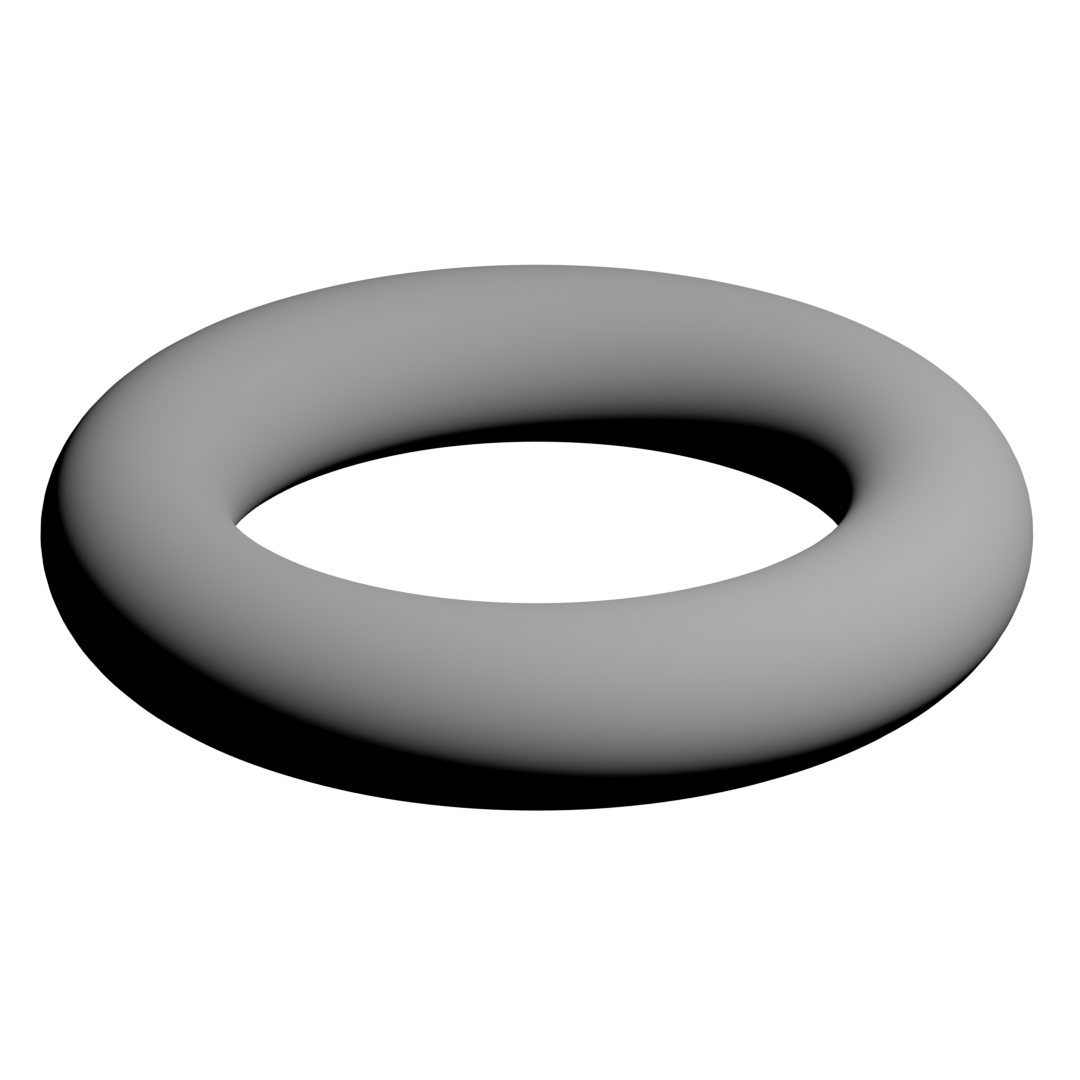
\includegraphics[scale=\myscale,scale=0.13, trim={0 6cm 0 4cm}, clip]{figures/tore-diffuse}
		
		{\bf \quad Lumière diffuse}
	\end{minipage}
	\begin{minipage}{0.32\textwidth}
		\center
		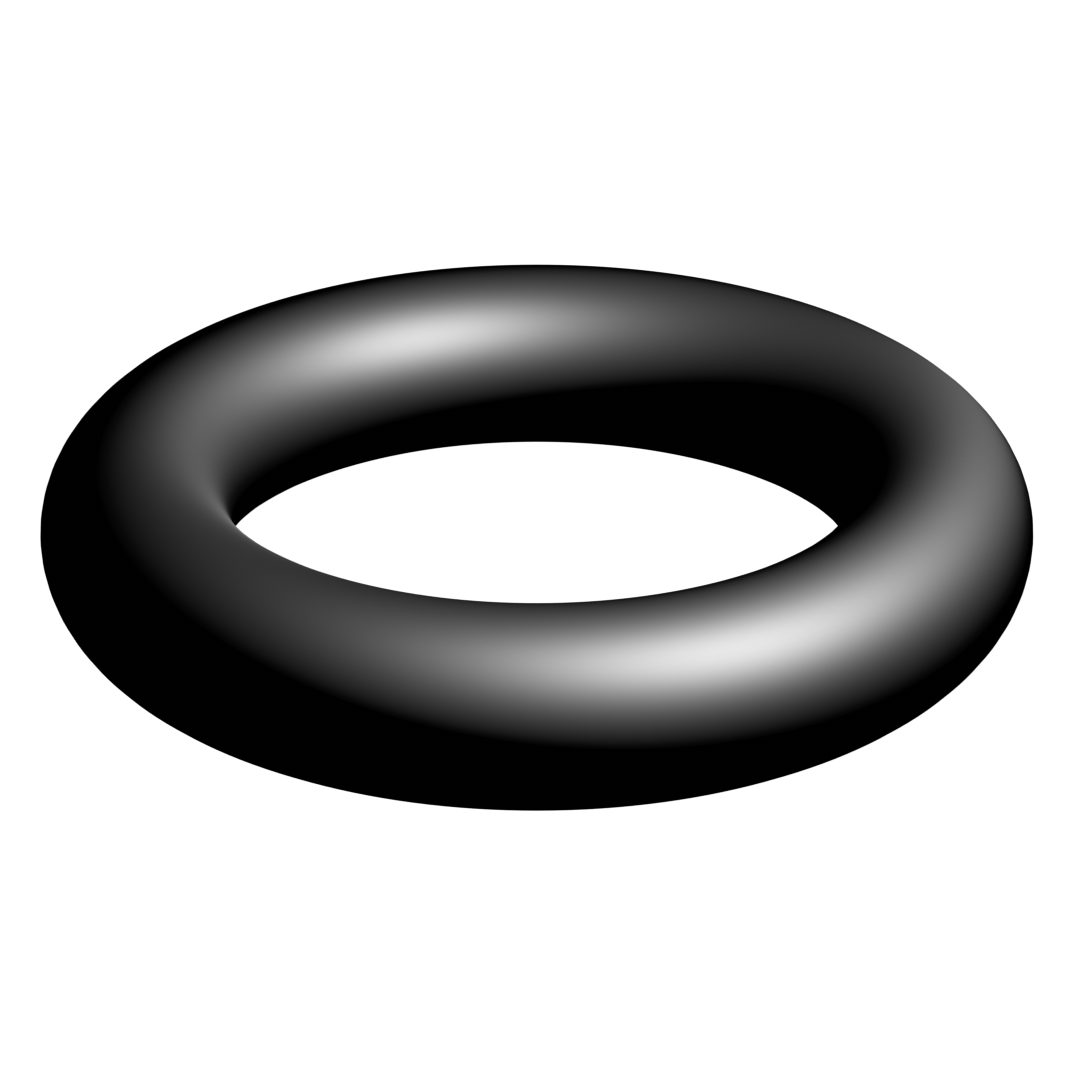
\includegraphics[scale=\myscale,scale=0.13, trim={0 6cm 0 4cm}, clip]{figures/tore-speculaire}
		
		{\bf \quad Lumière spéculaire}
	\end{minipage}
	
	\begin{minipage}{0.49\textwidth}
		\center
		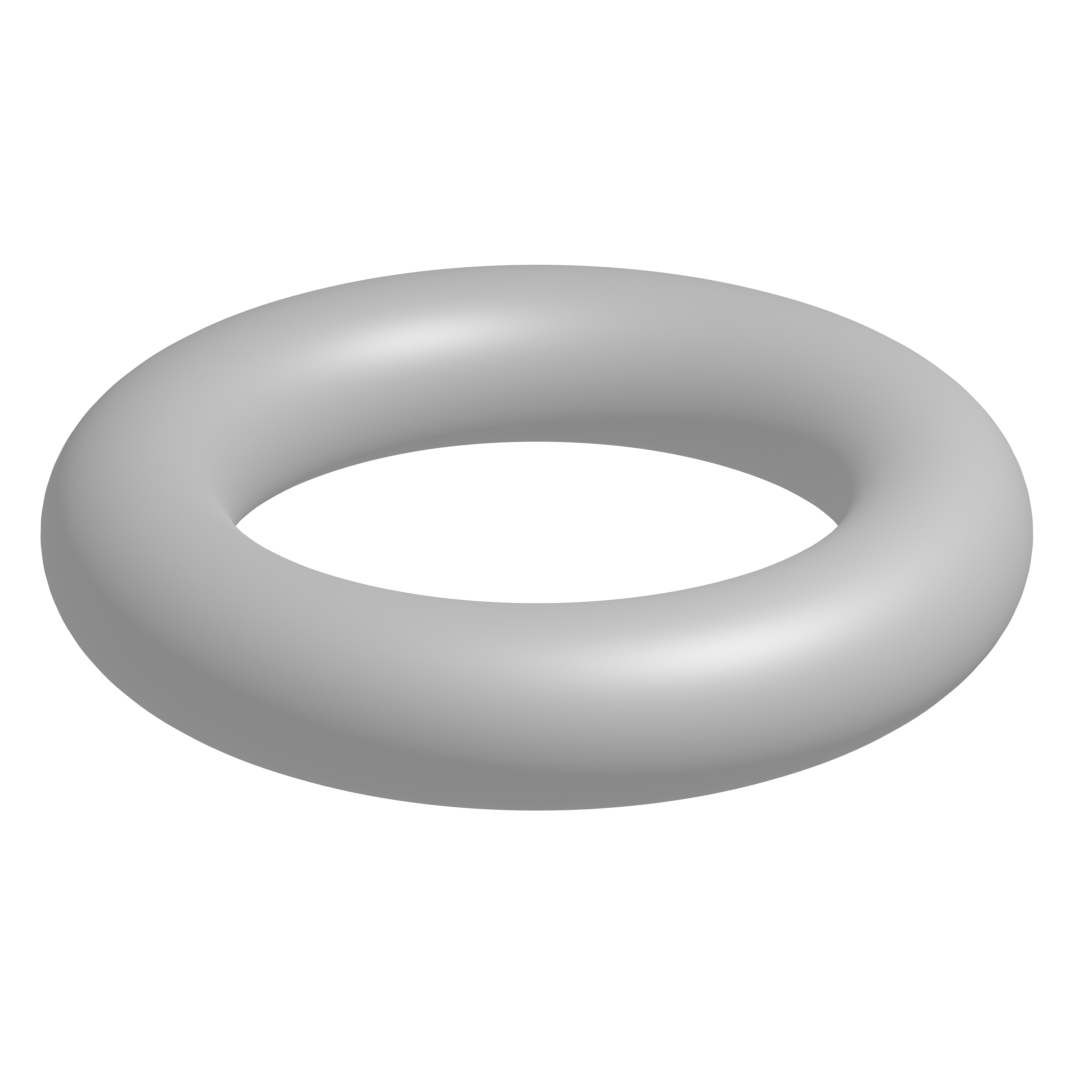
\includegraphics[scale=\myscale,scale=0.17, trim={0 6cm 0 4cm}, clip]{figures/tore-ambiante-diffuse-speculaire}
		
		{\bf \quad Lumière diffuse, ambiante et spéculaire}
	\end{minipage}
	
\end{center}


\textbf{Luminosité ambiante.}

La \defi{luminosité ambiante} correspond à une lumière qui n'a pas de source précise et éclaire partout, et dans toutes les directions, de la même façon.

\myfigure{0.5}{\tikzinput{fig-lumiere-14}}

La couleur perçue $\Cl_{\text{amb}}$ dépend de la couleur $\Cl_{\text{source}}$ et de l'intensité $i_{\text{source}}$ de l'éclairage, mais aussi de la couleur propre de l'objet $\Cl_{\text{objet}}$ :
\mybox{$\displaystyle \Cl_{\text{amb}} = i_{\text{source}} \Cl_{\text{source}} \otimes_{cl} \Cl_{\text{objet}}$}


On rappelle que l'addition de deux couleurs, notée par $\oplus_{cl}$, se fait en ajoutant terme à terme les composantes $r,g,b$, sans dépasser $1$.
La multiplication, notée $\otimes_{cl}$, s'effectue en  multipliant terme à terme les composantes $r,g,b$.
  
\medskip
  
\textbf{Luminosité diffuse.}

La \defi{luminosité diffuse} est une caractéristique associée aux matériaux mats et conduit à une réflexion de la lumière dans toutes les directions. Par contre, l'intensité des rayons réfléchis dépend de l'orientation de la surface par rapport au rayon lumineux.

\myfigure{0.5}{\tikzinput{fig-lumiere-16}}

La formule de la couleur diffuse est résumée en :
\mybox{$\displaystyle \Cl_{\text{diff}} = i_{\text{source}} \max(\vec\ell\cdot\vec n,0) \Cl_{\text{source}} \otimes_{cl} \Cl_{\text{objet}}$}
où $i_{\text{source}}$ et $\Cl_{\text{source}}$ sont l'intensité et la couleur de la source lumineuse et $\Cl_{\text{objet}}$ est la couleur propre de l'objet.

\medskip

\textbf{Luminosité spéculaire.}

La \defi{luminosité spéculaire} s'observe sur les objets brillants, les rayons lumineux se réfléchissent autour de l'axe principal de réflexion. La couleur perçue par luminosité spéculaire dépend de la position de l'observateur $O$.


\myfigure{0.5}{\tikzinput{fig-lumiere-24}}


\mybox{$\displaystyle \Cl_{\text{spec}} 
	= i_{\text{source}} \; (\vec r\cdot\vec v)^{e_{\text{spec}}} \;
	\Cl_{\text{source}} \otimes_{cl} \Cl_{\text{objet}} $}

La formule dépend :
\begin{itemize}
	\item de l'intensité $i_{\text{source}}$ et la couleur $\Cl_{\text{source}}$ de la source lumineuse mais aussi de la couleur $\Cl_{\text{objet}}$ propre à l'objet, 
	\item de l'axe principal de réflexion $\vec r$,
	\item de la direction $\vec v$ vers l'observateur,
	\item d'un exposant d'étalement $e_{\text{spec}}$.
\end{itemize}

L'axe principal de la réflexion $\vec r$ est le vecteur symétrique de $\vec\ell$ (qui pointe vers la source lumineuse) par rapport à $\vec n$ (orthogonal à la surface).

\myfigure{0.6}{\tikzinput{fig-lumiere-23}}


\medskip

\textbf{Éclairage direct.}
Cette couleur perçue, obtenue comme somme des trois composantes ambiante, diffuse, spéculaire, sera par la suite appelée la couleur obtenue par \defi{éclairage direct}.
Pour un point $P$ d'un objet, observé depuis un point $O$, cette couleur sera notée :
\mybox{$\displaystyle \Cl^{\text{dir}}_{P (\leftarrow O)}$}

La flèche dans la notation \og{}$P (\leftarrow O)$\fg{} est dans le même sens que le rayon du \emph{ray-tracing} qui va de l'observateur $O$ vers le point $P$ de l'objet (attention cette flèche va à rebours du rayon lumineux).


\medskip

Nous allons maintenant apporter des améliorations à la version simplifiée du \emph{ray-tracing} expliquée auparavant.



%--------------------------------------------------------------------
\subsection{Ombre et sources lumineuses}

Le dernier rayon, lancé du point $P$ de l'objet vers la source lumineuse $S$ s'appelle le \defi{rayon d'ombre}\index{rayon d'ombre} (\emph{shadow ray}).


\myfigure{0.6}{
	\tikzinput{fig-ombre-01}
}

 En effet, il se peut qu'un autre objet soit intercalé entre $P$ et $S$. Si cet objet est opaque cela signifie que la source lumineuse est obstruée, autrement dit un rayon lumineux issu de $S$ n'atteint pas le point $P$ ; vous êtes dans l'ombre de l'objet et il n'y a pas d'éclairage direct ; en l'absence de toute autre source lumineuse, la couleur associée à ce point $P$ est alors le noir.
En général, on ajoute toujours une composante de lumière ambiante, ce qui fait que même un objet à l'ombre sera légèrement visible.


\myfigure{0.7}{
	\tikzinput{fig-ombre-02}
}


S'il y a plusieurs sources lumineuses, il faut lancer un rayon depuis $P$ vers chacune des sources lumineuses $S_1$, $S_2$\ldots{} 
La couleur en $P$ est alors la somme (au sens du chapitre \og{}Lumière\fg{}) des couleurs résultant de chaque source.

\myfigure{0.6}{
	\tikzinput{fig-ombre-03}
}


Une source lumineuse peut ne pas être réduite à un point, cela peut être un disque (comme le Soleil apparent) ou un rectangle (comme un projecteur carré). Chaque point de cette surface peut être considéré comme une source de lumière ponctuelle ou directionnelle.
L'intensité de la lumière qui atteint l'objet en un point $P$ est proportionnelle à la surface visible de la source lumineuse depuis ce point.


\myfigure{0.8}{
	\tikzinput{fig-ombre-04}
}

Ci-dessous, ligne du haut : (a) une source lumineuse sans lumière ambiante, (b) une source lumineuse avec une lumière ambiante.
Ligne du bas : (c) deux sources lumineuses, (d) une source lumineuse non ponctuelle.

\begin{center}
	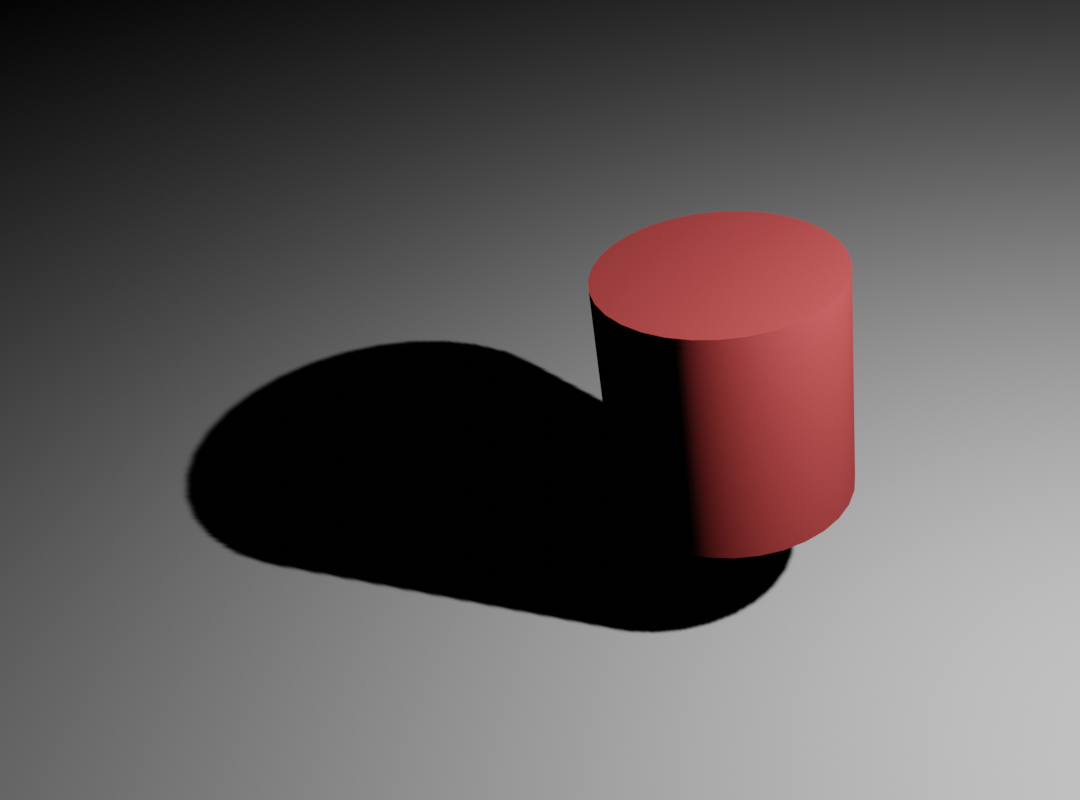
\includegraphics[scale=\myscale,scale=0.2,trim={2cm 2cm 2cm 2cm},clip]{figures/ombre-brute}
	\qquad
	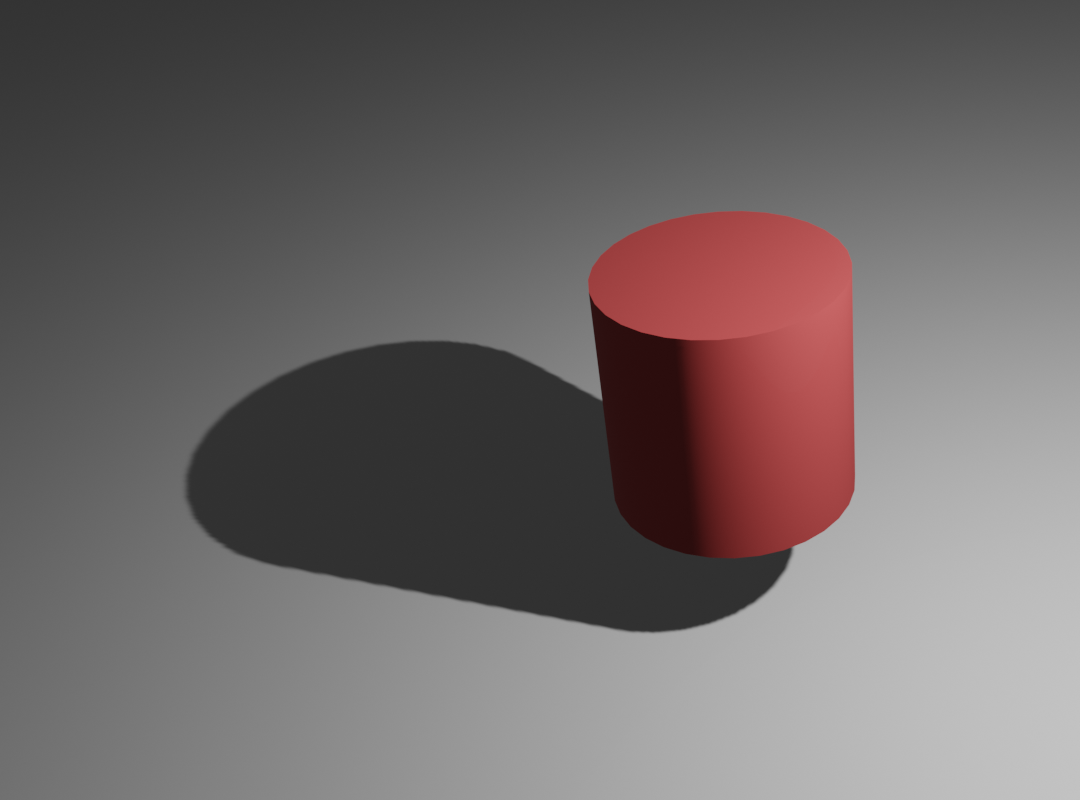
\includegraphics[scale=\myscale,scale=0.2,trim={2cm 2cm 2cm 2cm},clip]{figures/ombre-ambiante}
\end{center}	

\begin{center}
	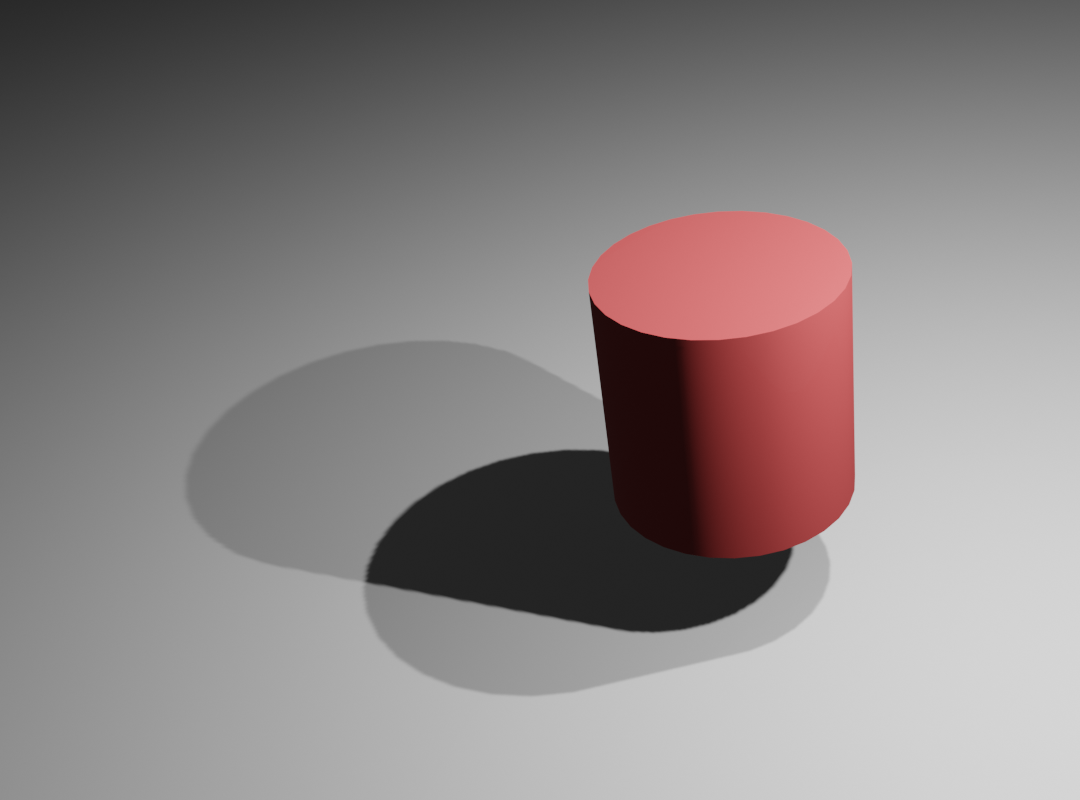
\includegraphics[scale=\myscale,scale=0.20,trim={2cm 2cm 2cm 2cm},clip]{figures/ombre-deux}	
	\qquad
	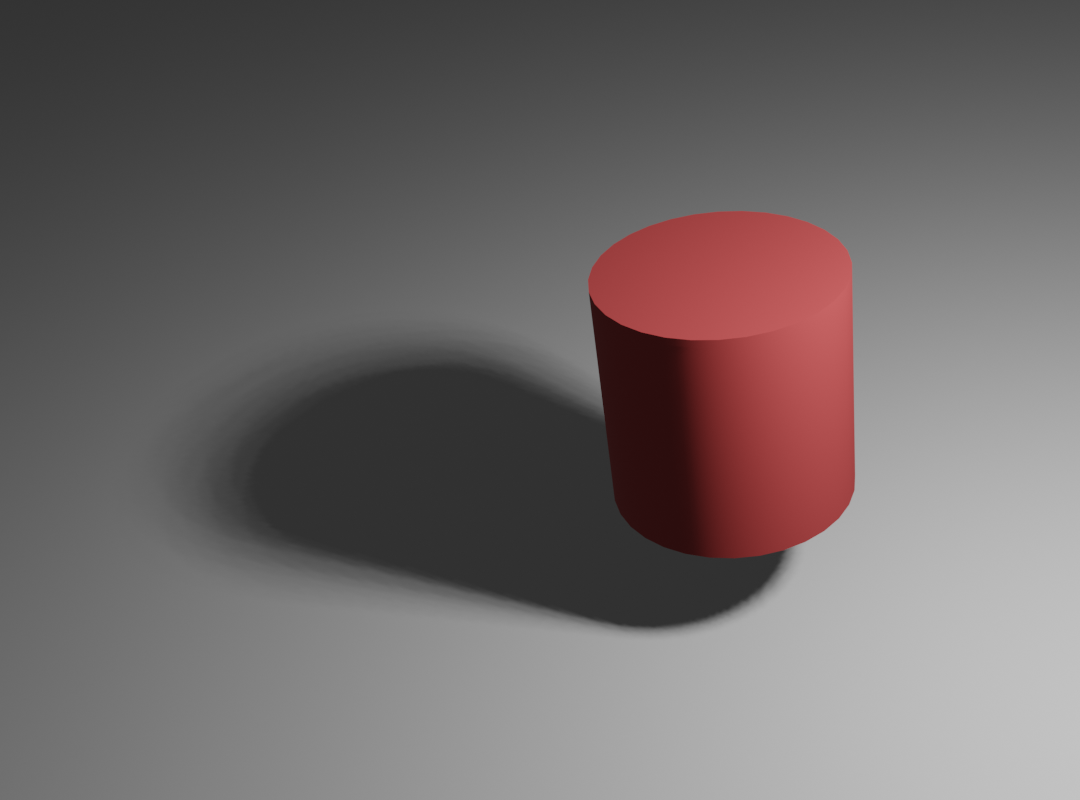
\includegraphics[scale=\myscale,scale=0.20,trim={2cm 2cm 2cm 2cm},clip]{figures/ombre-surface}
\end{center}





%--------------------------------------------------------------------
\subsection{Réflexions multiples}

Le \emph{ray-tracing} prend toute sa force lorsqu'on considère les réflexions multiples qui donnent un éclairage indirect. Ainsi chaque objet peut être une source lumineuse pour les autres objets.


\myfigure{0.8}{
	\tikzinput{fig-multiples-01}
}

Dans la situation ci-dessus, le point $P$ de l'objet $\mathcal{O}_1$ est éclairé de deux façons : 
\begin{itemize}
	\item par éclairage direct via un rayon issu de $P$ dirigé vers $S$ (comme auparavant),
	\item par éclairage indirect via l'objet $\mathcal{O}_2$.
\end{itemize}

Expliquons comment calculer la composante issue de l'éclairage indirect.

\begin{enumerate}
	\item On lance un rayon $\vec{r_0}$ issu de $O$, on calcule le premier point $P$ d'intersection avec un objet de la scène.
	
	\item On calcule la luminosité associée à la lumière directe $\Cl^{\text{dir}}_{P(\leftarrow O)}$ (en lançant un rayon de $P$ vers $S$).
	
	\item On calcule le rayon $\vec{r_1}$ obtenu par une réflexion parfaite de $\vec{r_0}$ selon la normale en $P$. On calcule le premier point $Q$ d'intersection de $\vec{r_1}$ avec un objet de la scène.
	
	\item On calcule la luminosité associée à la lumière directe en $Q$ perçue depuis $P$ : $\Cl^{\text{dir}}_{Q(\leftarrow P)}$ (en lançant un rayon de $Q$ vers $S$).	
	
	\item On calcule la composante de luminosité indirecte en $P$ issue de $Q$ comme une fraction de la composante précédente : $\Cl^{\text{indir}}_{P(\rightarrow Q)} = k_Q \Cl^{\text{dir}}_{Q(\leftarrow P)}$ où $k_Q$ est un coefficient, appelé \emph{facteur de réflexivité}.	 
	
	\item La luminosité totale perçue en $P$ est la somme de la luminosité directe et indirecte :
	$\Cl_P = \Cl^{\text{dir}}_{P} \oplus_{cl}\Cl^{\text{indir}}_{P}$.
\end{enumerate}

Souvenez-vous que les flèches \og{}$\rightarrow$\fg{} et  \og{}$\leftarrow$\fg{} indiquent le sens des rayons du \emph{ray-tracing}.


\myfigure{0.8}{
	\tikzinput{fig-multiples-02}
}

Ci-dessous à gauche, un cube avec un éclairage orienté vers le côté droit, la face du dessus et celle de gauche ne sont pas éclairées.
Sur la figure de droite, on rajoute une sphère qui réfléchit la lumière, la face supérieure du cube est alors éclairée par une lumière indirecte.
\begin{center}
	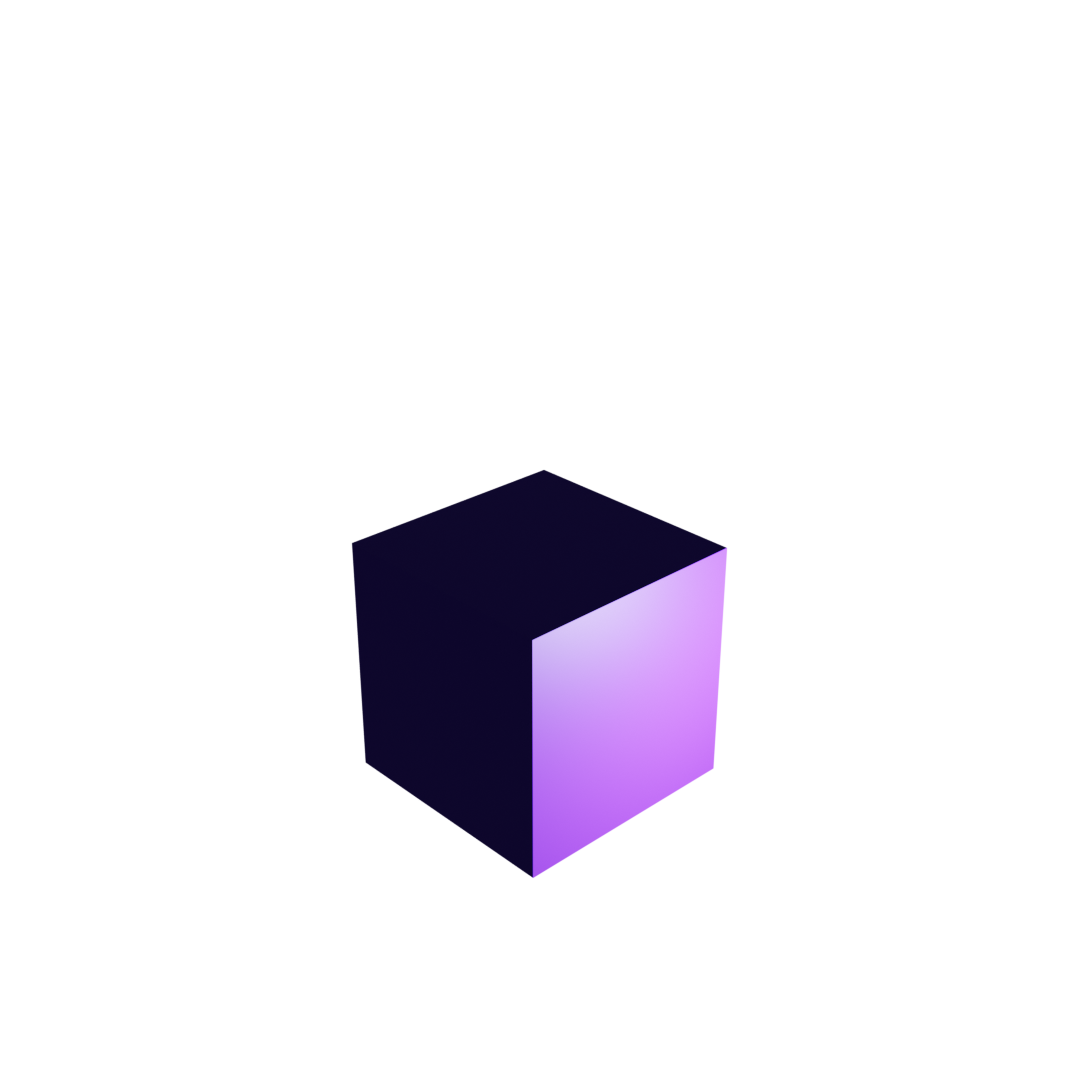
\includegraphics[scale=\myscale,scale=0.25,trim={4cm 2cm 4cm 2cm},clip]{figures/ray-tracing-01-1}
	\qquad
	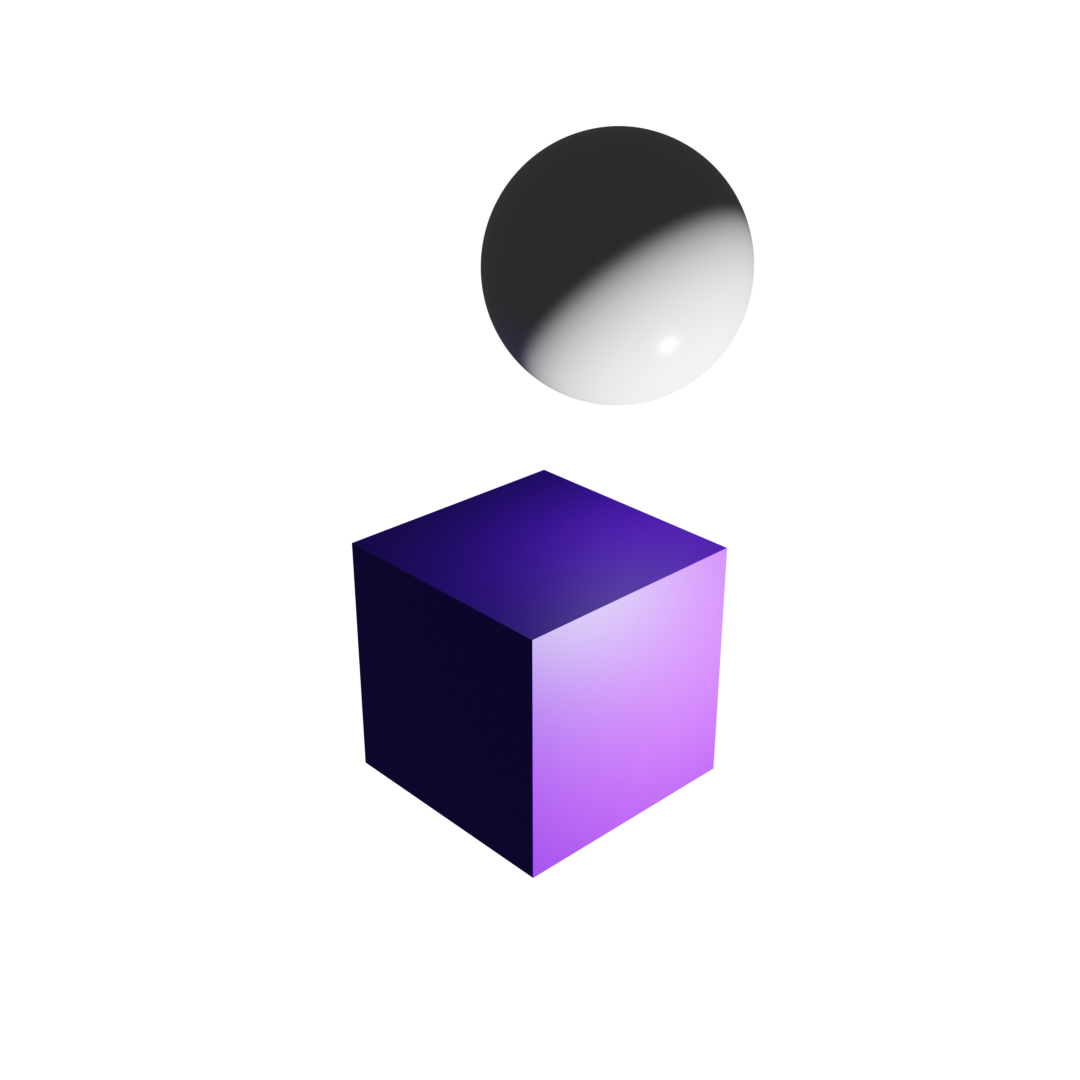
\includegraphics[scale=\myscale,scale=0.25,trim={4cm 2cm 4cm 2cm},clip]{figures/ray-tracing-01-2}
\end{center}	


\medskip

 

%S'il y avait plusieurs sources de lumière indirecte, on aurait alors :
%$$\Cl_P = \Cl^{\text{dir}}_{P(\leftarrow O)} 
%\oplus_{cl} \Cl^{\text{indir}}_{P(\rightarrow Q_1)}
%\oplus_{cl} \Cl^{\text{indir}}_{P(\rightarrow Q_2)}	
%\oplus \cdots$$

\medskip

\textbf{Facteur de réflexivité.} Le coefficient $k_Q$ est un nombre réel entre $0$ et $1$ et dépend de la matière en $Q$. Un matériau absorbant aura un coefficient nul, un miroir aura un coefficient $1$.
Il est aussi important de garder à l'esprit qu'un rayon lumineux ne perd pas en intensité, quelle que soit la distance parcourue, tant qu'il ne rencontre pas d'obstacle.
Notez bien que le rayon indirect (de $P$ vers $Q$) est celui obtenu par réflexion parfaite.
On pourrait considérer que ce modèle n'est pas réaliste et que la lumière se diffuse en $Q$,
dans ce cas on diminue l'intensité perçue en $Q$ proportionnellement au carré de la distance $PQ$.

\medskip

\textbf{Couleur au point de réflexion.} 
Pour une meilleure modélisation il faut tenir compte de la couleur de la surface d'où provient la lumière indirecte. Ainsi une lumière blanche qui se réfléchit sur un objet vert en $Q$, va réfléchir une lumière verte vers $P$. Ceci est pris en compte dans le calcul de l'éclairage direct en $Q$, $\Cl^{\text{dir}}_{Q(\leftarrow P)}$ pour lequel les formules des luminosités ambiante, diffuse et spéculaire tiennent compte de la couleur de l'objet $\Cl_{\text{objet}}$ en $Q$.


\medskip

\textbf{Réflexions multiples.}
Dans les explications précédentes nous n'avons considéré qu'un seul rebond indirect (au point $Q$). Pour les réflexions multiples il faut itérer le processus à partir du point $Q$.
Sur le dessin ci-dessous la source lumineuse n'éclaire pas directement le point $P$, ni l'objet $\mathcal{O}_1$ (dans l'ombre), ni la face supérieure de l'objet $\mathcal{O}_2$. Seul l'objet $\mathcal{O}_3$ est éclairé directement.


\myfigure{0.8}{
	\tikzinput{fig-multiples-03}
}

Pour calculer l'éclairage indirect en $P$, vu de $O$ :
\begin{itemize}
	\item on lance un rayon $\vec{r_0}$ de $O$ vers $P$,
	\item par symétrie par rapport à la normale en $P$, on lance un rayon $\vec{r_1}$ de $P$ vers un point $Q_1$,
	\item par symétrie par rapport à la normale en $Q_1$, on lance un rayon $\vec{r_2}$ de $Q_1$ vers un point $Q_2$,
	\item par symétrie par rapport à la normale en $Q_2$, on lance un rayon $\vec{r_3}$ de $Q_2$ vers un point $Q_3$,
	\item depuis $Q_3$ on lance un rayon d'ombre $\vec{\ell_{Q_3}}$ vers la source lumineuse $S$.
\end{itemize}			
On remonte ensuite notre construction : on calcule la luminosité directe perçue en $Q_3$ (depuis $Q_2$) : $\Cl_{Q_3}$. Ainsi la luminosité indirecte perçue en $Q_2$ est $k_{Q_3}\Cl_{Q_3}$, celle en $Q_1$ est $k_{Q_2}k_{Q_3}\Cl_{Q_3}$ et au final la luminosité indirecte perçue en $P$ est :
$$\Cl^{\text{indir}}_{P} = k_{Q_1}k_{Q_2}k_{Q_3}\Cl_{Q_3}.$$
Dans cet exemple on a considéré que les objets intercalés ne changent pas la couleur de la lumière mais juste son intensité.
Nous étudierons la formule de récurrence générale juste après.
Comme chaque coefficient $k$ est inférieur à $1$, l'intensité de la lumière indirecte diminue à chaque réflexion et devient vite négligeable après $1$, $2$ ou $3$ réflexions.
Il existe cependant une exception : dans le cas d'un miroir parfait où $k=1$, on peut avoir (en théorie) une infinité de réflexions ; c'est un phénomène que vous avez sûrement déjà expérimenté en vous plaçant entre deux miroirs parallèles.


%--------------------------------------------------------------------
\subsection{Transparence}

\index{transparence}

Nous allons étudier la propriété de transparence.
Ci dessous : (a) deux tores opaques, (b) un seul tore transparent (sans changement milieu), (c) un tore est en verre (d'indice $n \simeq 1.4$). 
\begin{center}
	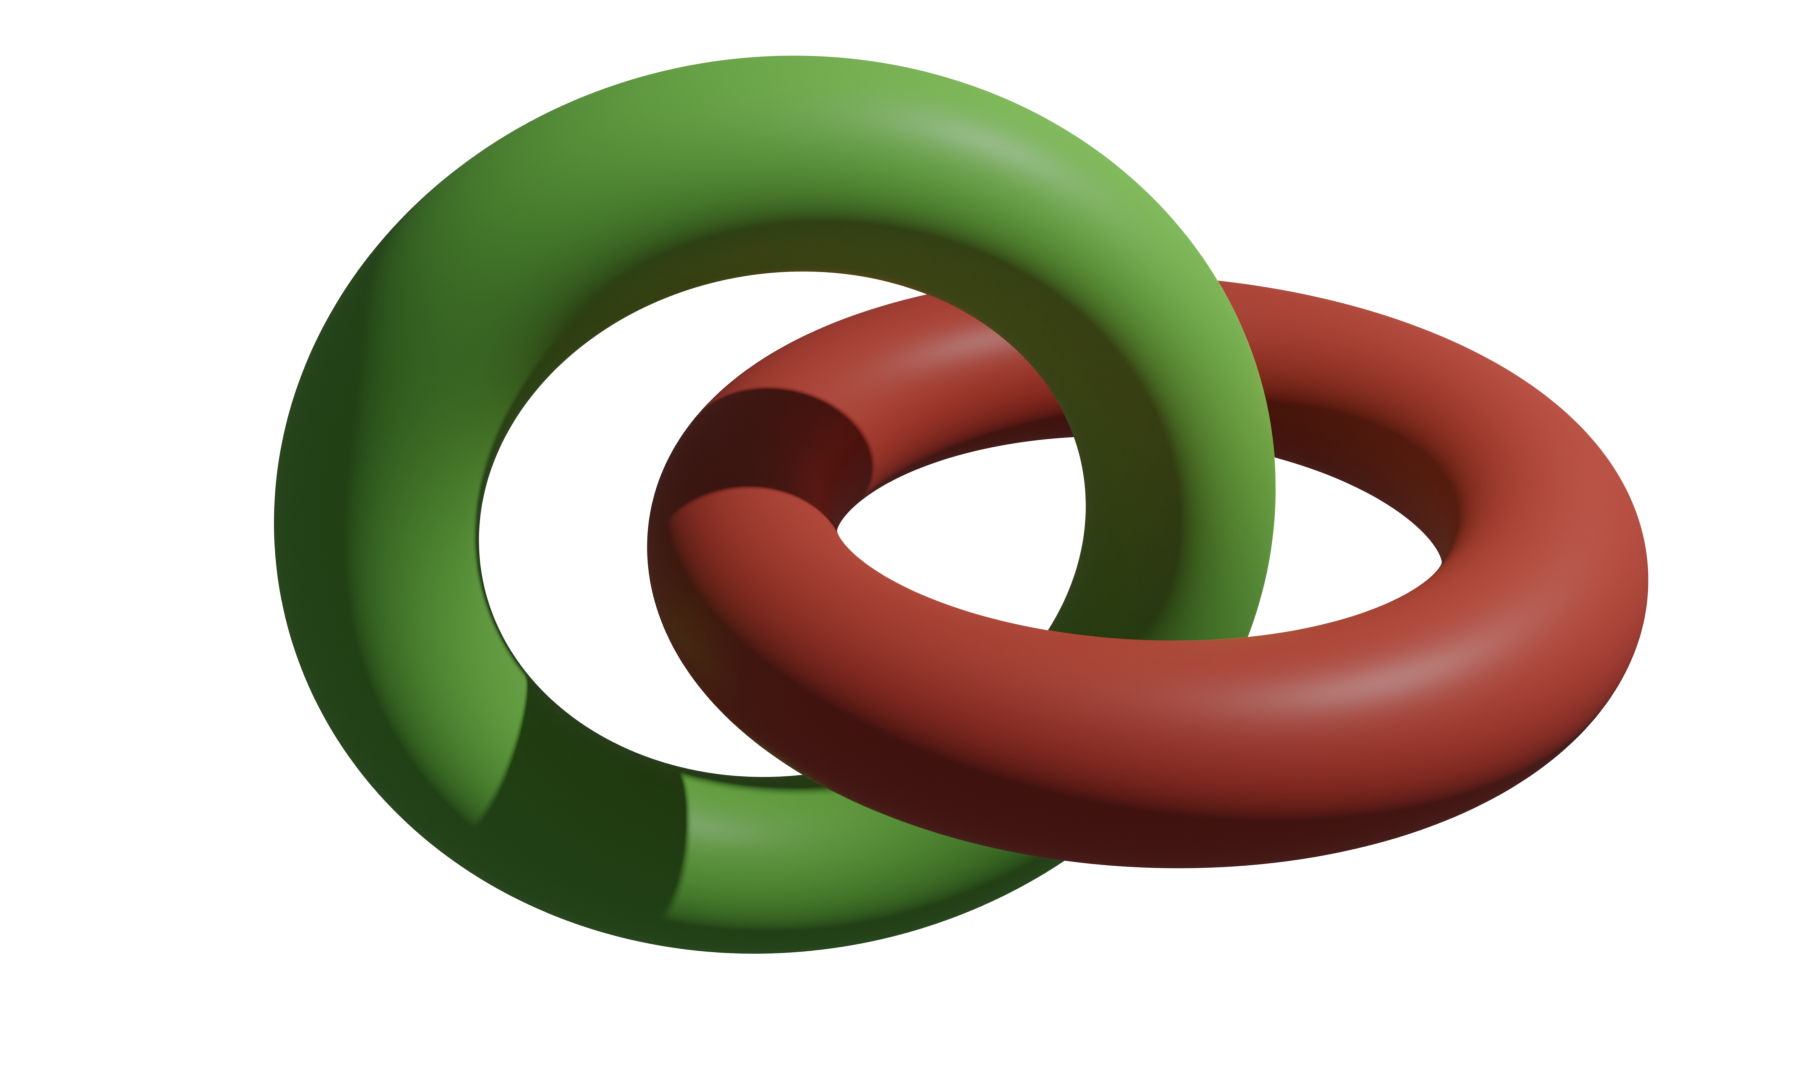
\includegraphics[scale=\myscale,scale=0.1,trim={6cm 2cm 4cm 0cm},clip]{figures/ray-tracing-02-1}
	\quad
	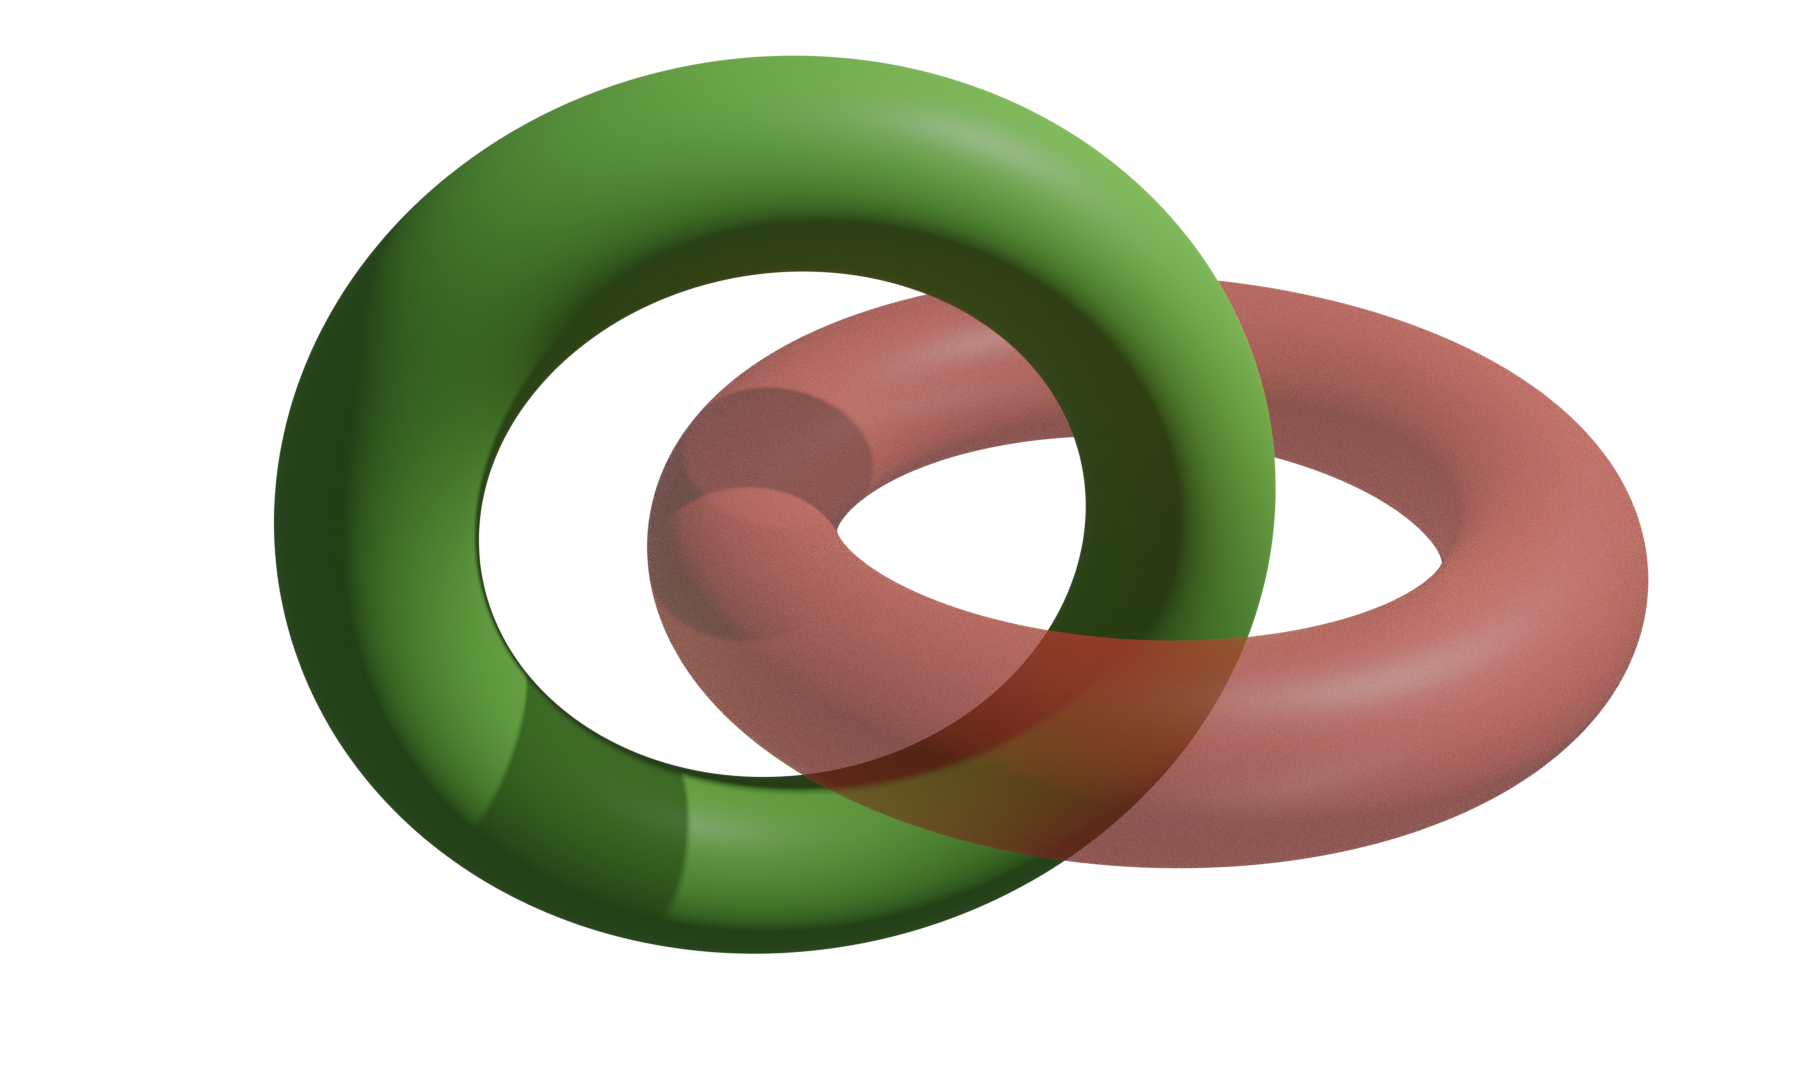
\includegraphics[scale=\myscale,scale=0.1,trim={8cm 2cm 4cm 0cm},clip]{figures/ray-tracing-02-2}
	\quad
    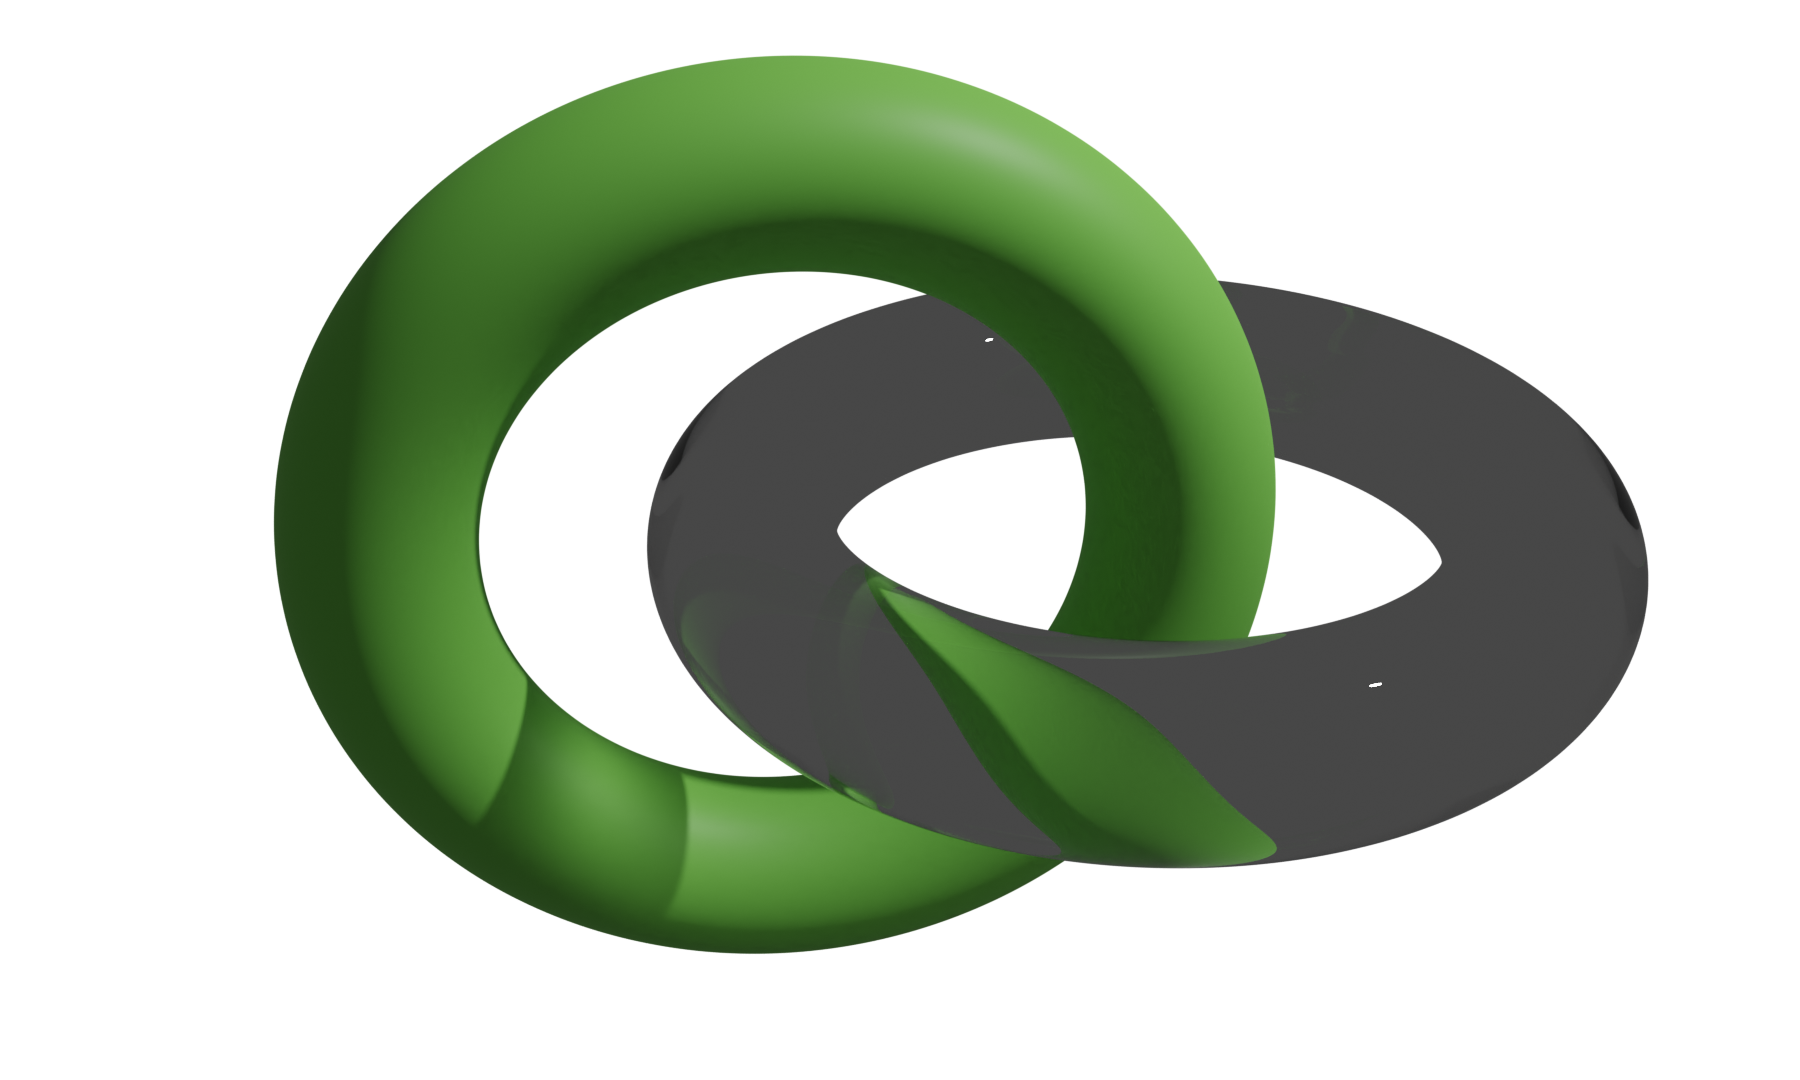
\includegraphics[scale=\myscale,scale=0.1,trim={4cm 2cm 4cm 0cm},clip]{figures/ray-tracing-02-3}	
\end{center}

Nous avons déjà étudié la \defi{réflexion}\index{lumiere@lumière!reflexion@réflexion} d'un rayon dans le chapitre \og{}Lumière\fg{} :
un rayon arrivant sur une surface rebondit dans la direction symétrique par rapport à la normale.

\begin{minipage}{0.49\textwidth}
	\myfigure{0.7}{
		\tikzinput{fig-transparence-01}
	}  
\end{minipage}	
\begin{minipage}{0.49\textwidth}
	\myfigure{0.6}{
	    \tikzinput{fig-transparence-02}
    } 	
\end{minipage}

\medskip

Nous étudierons plus tard la \defi{réfraction}\index{lumiere@lumière!refraction@réfraction} (voir la chapitre \og{}Physique\fg{}) : lorsqu'un rayon change de milieu, par exemple il passe de l'air à l'eau ou bien traverse du verre, sa trajectoire est déviée. L'angle de déviation est régi par la loi de Snell-Descartes\index{loi!de Snell-Descartes} :
$$n_1 \sin \theta_1 = n_2 \sin \theta_2$$
où $n_1$ et $n_2$ sont les \emph{indices} qui dépendent du milieu (mais aussi de la longueur d'onde du rayon).

Pour un matériau transparent, par exemple du verre, les deux phénomènes se produisent : une partie du rayon est réfléchie, l'autre est réfractée. De plus une partie de l'énergie du rayon est absorbée par le matériau (ce qui se traduit dans nos calculs par le facteur $k \le 1$).

\myfigure{0.6}{
	\tikzinput{fig-transparence-03}
} 

%Par le principe de conservation de l'énergie : $i_0 = i_1 + i_2$, c'est-à-dire l'intensité lumineuse du rayon incident est égale à la somme des intensités du rayon réfléchi et du rayon réfracté.

\textbf{Conclusion.} Dorénavant lorsqu'un rayon atteint un objet ayant des propriétés de transparence il faut relancer deux rayons depuis le point d'impact : un rayon réfléchi et un rayon réfracté.



Il y a une exception que l'on fera : lorsqu'on lance le rayon d'ombre $\vec{\ell_P}$, on considère qu'il se dirige tout droit vers la source lumineuse, si ce rayon rencontre un objet translucide on peut éventuellement atténuer la luminosité.

\myfigure{0.6}{
	\tikzinput{fig-ombre-05}
} 


\begin{exercicecours}
\sauteligne
\begin{enumerate}
	\item Sur la figure de gauche ci-dessous, tracer les rayons correspondant à l'éclairage direct d'un point de la surface du lac, puis faire la même chose avec un point de la surface de la montagne.
\myfigure{0.6}{
	\tikzinput{fig-lac-01}
} 	
	\item Sur la figure de gauche ci-dessous, tracer les rayons correspondant à l'éclairage indirect d'un point de la surface du lac où apparaît le reflet de la montagne.
	
\myfigure{0.6}{
	\tikzinput{fig-lac-02}
} 
	
	\item Sur la figure de gauche ci-dessous, tracer les rayons correspondant à l'éclairage du poisson par transparence.
	
\myfigure{0.6}{
	\tikzinput{fig-lac-03}
}
	
\end{enumerate}
	
\end{exercicecours}


\medskip

\textbf{Complications.}

\emph{Paroi.} Lorsque le rayon traverse une paroi de verre alors il faut appliquer ce principe des deux côtés de la paroi. Noter que le rayon traversant la paroi ressort parallèlement au rayon incident.

\myfigure{0.6}{
	\tikzinput{fig-transparence-04}
} 


\emph{Réflexion totale.} Lorsqu'on lance un rayon sous l'eau avec un angle faible par rapport à l'horizontale le comportement est différent : le rayon est complètement réfléchi, c'est le phénomène de \defi{réflexion totale} que vous pouvez observer du fond de l'eau en levant la tête vers la surface qui a alors l'allure d'un miroir.


\myfigure{0.8}{
	\tikzinput{fig-transparence-05}
} 

Ces phénomènes de réflexion/réfraction expliquent la formation des arcs-en-ciel, en effet les rayons se réfractent différemment selon leur couleur. La lumière blanche du Soleil, constituée de rayons de toutes les couleurs, entre dans une goutte d'eau, les rayons sont plus ou moins réfractés selon leur longueur d'onde, il y a ensuite une réflexion interne à la goutte puis une nouvelle réfraction qui sépare davantage les rayons.
On retrouvera ce phénomène dans le chapitre \og{}Physique\fg{} avec l'expérience du prisme de Newton.


\myfigure{1.5}{
	\tikzinput{myrainbow}
} 


%--------------------------------------------------------------------
\subsection{Mise en \oe uvre}

\index{algorithme!du ray-tracing@du \emph{ray-tracing}}

Expliquons les grandes lignes de l'algorithme de \emph{ray-tracing}.
C'est un excellent projet de le programmer mais cela demande plusieurs jours de travail.
Ci-dessous une scène avec cinq objets, dont un transparent, devant un miroir, avec deux sources lumineuses.
\begin{center}
	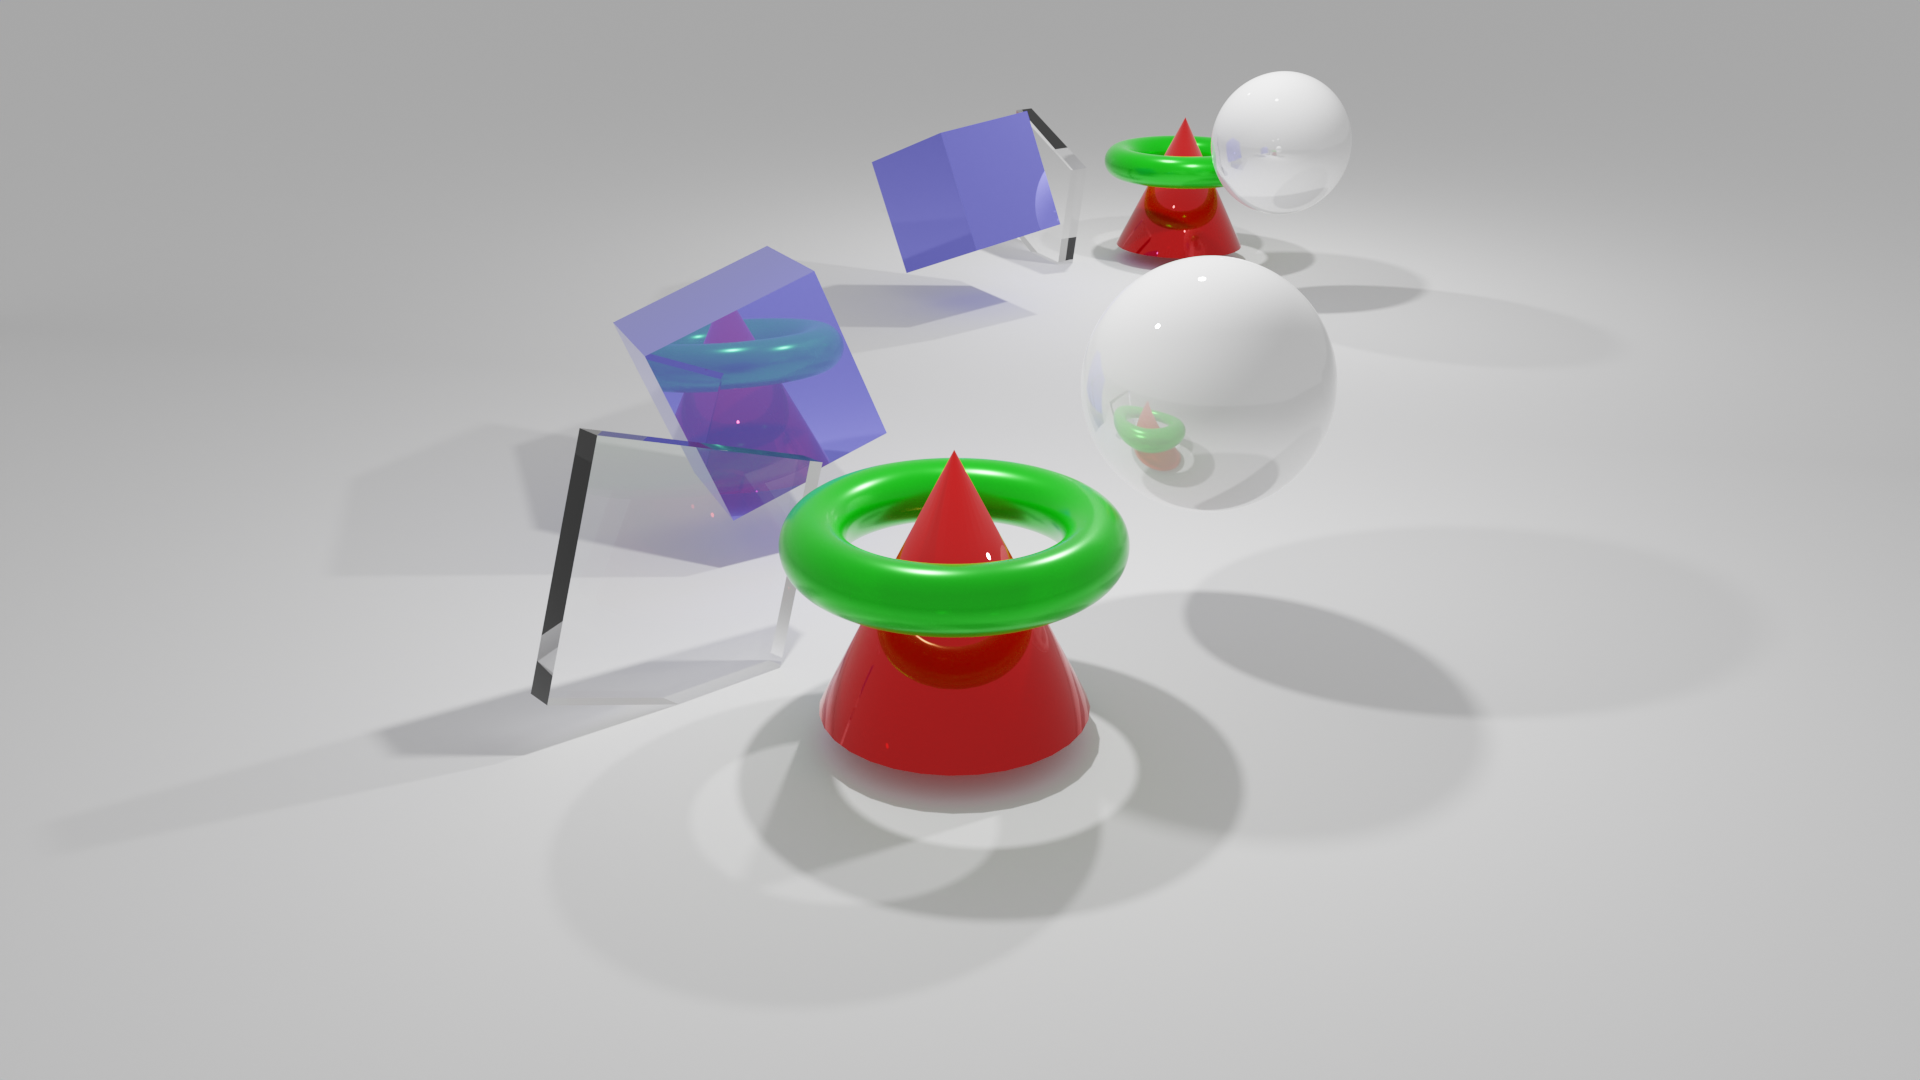
\includegraphics[scale=\myscale,scale=0.30,trim={8cm 5cm 8cm 0cm},clip]{figures/ray-tracing-03}	
\end{center}


Au préalable nous devons disposer de :
\begin{itemize}
	\item une fonction \ci{lancer_rayon(O,r)} qui calcule les points d'intersection d'un rayon $\vec{r_0}$ issu de $O$ avec les objets de la scène et renvoie le point $P$ le plus proche,
	\item une fonction \ci{couleur_directe(P,O)} qui renvoie la couleur $\Cl^{\text{dir}}_{P(\leftarrow O)}$ en $P$ perçue de $O$, obtenue par addition des couleurs ambiante, diffuse et spéculaire.
\end{itemize}


On souhaite attribuer une couleur au pixel $E_{ij}$ de l'écran,
pour cela on calcule le rayon $\vec{r_0}$ de $O$ vers $E_{ij}$.
On note $P$ le premier point d'intersection de $\vec{r_0}$ avec la scène,
si le rayon ne coupe aucun objet on colorie le pixel par la couleur de fond.

Il s'agit ensuite de définir une fonction \ci{couleur(P,O)} qui calcule la couleur $\Cl_{P(\leftarrow O)}$ obtenue par \emph{ray-tracing}. Cette fonction est une fonction récursive (elle s'appelle elle-même).


\medskip

Structure de \ci{couleur(P,O)} :
\begin{enumerate}
	\item On teste la condition d'arrêt.
	\item On calcule la couleur directe $\Cl^\text{dir}_{P(\leftarrow O)}$ en $P$ perçue de $O$.
	\item on note $\vec{r_0}$ le rayon de $O$ vers $P$ et $\vec{r_1}$ le rayon obtenu par réflexion parfaite en $P$ ; on calcule $Q_1$ le premier point d'intersection de $\vec{r_1}$ avec la scène.
	\item Par un appel récursif \ci{couleur(Q1,P)}, on calcule la couleur $\Cl_{Q_1(\leftarrow P)}$ en $Q_1$ perçue depuis $P$.
	\item On calcule la couleur indirecte en $P$ issue de $Q_1$ :
	$$\Cl^{\text{indir}}_{P(\rightarrow Q_1)} = k_{Q_1} \Cl_{Q_1(\leftarrow P)}.$$
    \item Si l'objet a des propriétés de transparence on note $\vec{r_2}$ le rayon obtenu par réfraction de $\vec{r_0}$ en $P$, on calcule $Q_2$ le premier point d'intersection de $\vec{r_2}$ avec la scène.
    \item Par un appel récursif \ci{couleur(Q2,P)} on calcule la couleur $\Cl_{Q_2(\leftarrow P)}$ en $Q_2$ perçue depuis $P$.
   \item On calcule la couleur indirecte en $P$ issue de $Q_2$ :
   $$\Cl^{\text{indir}}_{P(\rightarrow Q_2)} = k_{Q_2} \Cl_{Q_2(\leftarrow P)}.$$	
   \item On renvoie la couleur $\Cl_{P(\leftarrow O)}$ comme somme de la couleur directe et des couleurs indirectes :
   $$\Cl_{P(\leftarrow O)} = \Cl^{\text{dir}}_{P(\leftarrow O)} 
   \oplus_{cl} \Cl^{\text{indir}}_{P(\rightarrow Q_1)}
   \oplus_{cl} \Cl^{\text{indir}}_{P(\rightarrow Q_2)}.$$	
\end{enumerate}

\myfigure{0.6}{
	\tikzinput{fig-ray-tracing}
} 

	
\textbf{Condition(s) d'arrêt.}
Les rayons pouvant rebondir une infinité de fois, la condition d'arrêt est importante. La condition la plus simple est de définir à l'avance un nombre maximal de rebonds possibles, autrement dit de limiter la profondeur des appels récursifs.
On peut en plus stopper le processus dès que la luminosité indirecte va être faible et ne contribue presque plus à l'éclairement. On peut par exemple arrêter les appels récursifs dès que le produit des constantes de réflexivité est suffisamment petit : $k_{Q_{i_1}} k_{Q_{i_2}} \cdots k_{Q_{i_n}} \le \epsilon$.

\medskip

\textbf{Arbre de récursivité.}
L'arbre suivant montre la succession des points où il faut calculer la lumière directe afin d'obtenir l'éclairage indirect en $P$.

\myfigure{0.6}{
	\tikzinput{fig-arbre}
} 


%%%%%%%%%%%%%%%%%%%%%%%%%%%%%%%%%%%%%%%%%%%%%%%%%%%%%%%%%%%%%%%%%%%%%
\section{Intersection efficace avec un triangle}

Dans le chapitre \og{}Lancer de rayons I\fg{} nous avons vu comment calculer l'intersection d'un rayon avec des objets géométriques simples. Les figures géométriques les plus importantes sont les triangles de l'espace qui correspondent aux faces d'un maillage triangulaire. Nous allons donc calculer plus efficacement l'intersection d'un rayon avec un triangle.


%--------------------------------------------------------------------
\subsection{Rayon lancé sur un triangle}


Considérons un triangle de l'espace défini par trois points $A$, $B$, $C$ non alignés.
On lance un rayon issu de $S$ dans la direction $\vec v$. On suppose que le rayon n'est pas parallèle au plan $\mathcal{P}$ contenant le triangle.
Notons $P$ le point d'intersection du rayon avec ce plan $\mathcal{P}$.

\myfigure{1.1}{
	\tikzinput{fig-rayonsbis-triangle-01}
}  

Il existe donc $t \in \Rr$ tel que :
$$P = S + t \vec v$$
et comme $P$ est dans le plan $(ABC)$, il existe $u,v \in \Rr$ tels que :
$$P = A + u \overrightarrow{AB} + v \overrightarrow{AC}.$$
Le point $P$ est situé à l'intérieur (ou sur le bord) du triangle $ABC$ si et seulement si $0 \le u \le 1$ et $0 \le v \le 1$.
Pour les explications sur les coordonnées barycentriques $(1-u-v:u:v)$ on renvoie au chapitre \og{}Texture\fg{}.


\myfigure{0.5}{
	\tikzinput{fig-rayonsbis-triangle-02}
}  


Nous trouvons $t,u,v$ en résolvant le système linéaire de $3$ équations et $3$ inconnues, donné par :
$$S + t \vec v = A + u \overrightarrow{AB} + v \overrightarrow{AC}$$
En écrivant les coordonnées :
$$
\begin{pmatrix}x_S\\y_S\\z_S\end{pmatrix}
+ t \begin{pmatrix}x_v\\y_v\\z_v\end{pmatrix}
= \begin{pmatrix}x_A\\y_A\\z_A\end{pmatrix}
+ u \begin{pmatrix}x_B-x_A\\y_B-y_A\\z_B-z_A\end{pmatrix}
+ v \begin{pmatrix}x_C-x_A\\y_C-y_A\\z_C-z_A\end{pmatrix}.$$
Notons 
$$
M = 
\begin{pmatrix}
	x_v & -(x_B-x_A) & -(x_C-x_A) \\
	y_v & -(y_B-y_A) & -(y_C-y_A) \\
	z_v & -(z_B-z_A) & -(z_C-z_A) \\
\end{pmatrix}
\qquad\qquad
X = \begin{pmatrix}t\\u\\v\end{pmatrix} 
\qquad\qquad
Y = \begin{pmatrix}x_A-x_S\\y_A-y_S\\z_A-z_S\end{pmatrix}$$
Le système linéaire équivaut à l'équation matricielle, d'inconnue $X$ :
$$MX = Y.$$

On peut alors mettre en \oe uvre différentes techniques d'algèbre linéaire :
\begin{enumerate}
	\item calcul de l'inverse $M^{-1}$, puis $X = M^{-1}Y$,
	\item la méthode du pivot de Gauss,
	\item les formules de Cramer.
\end{enumerate}

C'est cette dernière méthode que nous allons détailler, mais auparavant rappelons comment calculer un déterminant.



%--------------------------------------------------------------------
\subsection{Déterminant $3\times 3$}

\index{determinant@déterminant}

Rappelons la formule du déterminant, uniquement dans le cas d'une matrice $3\times 3$.

Si $M$ est une matrice $3 \times 3$:
$$M = \begin{pmatrix}
	a_{11} & a_{12} & a_{13} \\
	a_{21} & a_{22} & a_{23} \\
	a_{31} & a_{32} & a_{33} \\
\end{pmatrix}$$
alors le déterminant se calcule selon la formule :
$$\det(M) =
a_{11} a_{22} a_{33}
+ a_{12} a_{23} a_{31}
+ a_{13} a_{21} a_{32}
- a_{31} a_{22} a_{13}
- a_{32} a_{23} a_{11}
- a_{33} a_{21} a_{12}\; .$$


Il existe d'autres façons de calculer un déterminant, on renvoie à un cours d'algèbre linéaire.

Rappelons cependant l'interprétation géométrique en termes de vecteurs.
Soient trois vecteurs de l'espace $\vec u, \vec v, \vec w$.
On forme la matrice $M$ de taille $3\times3$ en juxtaposant les vecteurs  $\vec u, \vec v, \vec w$ considérés comme des vecteurs colonnes. 

\begin{minipage}{0.45\textwidth}
\myfigure{1}{
	\tikzinput{fig-rayonsbis-triangle-04}
}
\end{minipage}
\begin{minipage}{0.45\textwidth}
\myfigure{1}{
	\tikzinput{fig-rayonsbis-triangle-03}	
}
\end{minipage}

\smallskip

Le déterminant de $M$, que l'on peut aussi noter $\det(\vec u, \vec v, \vec w)$, est égal au volume du parallélépipède formé par les trois vecteurs.



La formule du \defi{produit mixte} (\emph{triple product}) redonne aussi le déterminant:
$$\det(\vec u, \vec v, \vec w) = \vec u \cdot (\vec v \wedge \vec w).$$
Il faut donc d'abord calculer un produit vectoriel puis un produit scalaire. 
L'ordre des vecteurs est important pour le signe du déterminant.


%--------------------------------------------------------------------
\subsection{Méthode de Cramer}

La \defi{règle de Cramer}\index{regle de Cramer@règle de Cramer} est une formule qui donne la solution d'un système linéaire ayant autant d'équations que d'inconnues. On se contente de l'expliquer dans le cas $3 \times 3$.
Considérons le système d'équations linéaires à $3$ équations et $3$ inconnues suivant:
\[
\left\{
\begin{array}{ccc}
	a_{11} x_1 + a_{12} x_2 + a_{13} x_3 & = & y_1\\
	a_{21} x_1 + a_{22} x_2 + a_{23} x_3 & = & y_2\\
	a_{31} x_1 + a_{32} x_2 + a_{33} x_3 & = & y_3\\	
\end{array}
\right.
\]
Ce système peut aussi s'écrire sous forme matricielle $MX=Y$ où
$$
M = 
\begin{pmatrix}
	a_{11} & a_{12} & a_{13}\\
	a_{21} & a_{22} & a_{23}\\
	a_{31} & a_{32}& a_{33}
\end{pmatrix} \in M_{3}(\Rr), \qquad 
X = \begin{pmatrix} x_1\\x_2 \\x_3 \end{pmatrix}  \quad \text{et} \quad 
Y = \begin{pmatrix} y_1\\y_2\\y_3 \end{pmatrix}.
$$


Définissons les matrices $M_1, M_2, M_3$ en remplaçant la $j$-ème
colonne de $M$ par le second membre $Y$ :

 \myfigure{1}{
 	\tikzinput{fig-rayonsbis-triangle-05}	
 }

La règle de Cramer va nous
permettre de calculer la solution du système dans le cas où
$\det M \neq 0$ en fonction des déterminants des matrices $M$ et
$M_j$.

\begin{theoreme}[Règle de Cramer] 
	Soit $MX = Y$ un système de $3$ équations à $3$ inconnues. 
	Supposons que $\det M \neq 0$.
	Alors l'unique solution $(x_1,x_2,x_3)$ du système est donnée par:
	$$
	x_1 = \frac{\det M_1}{\det M} \qquad 
	x_2 = \frac{\det M_2}{\det M} \qquad
	x_3 = \frac{\det M_3}{\det M}.
	$$
\end{theoreme}

\begin{exemple} Résolvons le système suivant:
\[\left\{
\begin{array}{ccccccc}
	-2x_1 &+ &4x_2 &- &x_3 & = & 10\\		
	x_1 & && + &3x_3 & = &3\\
	x_1 &- &2x_2 &+ &3 x_3 & = & 4. \end{array}
\right. \]
On a
\[
M = \begin{pmatrix}
	-2 & 4 & -1\\
	1 & 0 & 3\\
	1 & -2 & 3
\end{pmatrix}
\qquad
Y = \begin{pmatrix}10 \\ 3 \\ 4 \end{pmatrix}
\]
\[
M_1 = \begin{pmatrix}
	10 & 4 & -1\\
	3 & 0 & 3\\
	4 & -2 & 3
\end{pmatrix}
\qquad
M_2 = \begin{pmatrix}
	-2 & 10 & -1\\
	1 & 3 & 3\\
	1 & 4 & 3
\end{pmatrix}
\qquad
M_3 = \begin{pmatrix}
	-2 & 4 & 10\\
	1 & 0 & 3\\
	1 & -2 & 4
\end{pmatrix}
\]
et
$$\det M  =  -10 \qquad \det M_1  = 78  \qquad
\det M_2  = 5  \qquad \det M_3  = -36.$$
La solution est alors :
\[
x_1 = \frac{\det M_1}{\det M} =  \frac{78}{-10}=  -\frac{39}{5}\qquad
x_2 = \frac{\det M_2}{\det M} =  \frac{5}{-10}=  -\frac{1}{2}\qquad
x_3 = \frac{\det M_3}{\det M} = \frac{-36}{-10}=  \frac{18}{5} \, \cdotp
\]
\end{exemple}



%%%%%%%%%%%%%%%%%%%%%%%%%%%%%%%%%%%%%%%%%%%%%%%%%%%%%%%%%%%%%%%%%%%%%
\section{Boites englobantes}

\index{boite englobante}

%--------------------------------------------------------------------
\subsection{Principe}

Calculer l'intersection d'un rayon avec un objet géométrique, ou même juste savoir si cette intersection existe, peut être coûteux en calculs. On renvoie par exemple au calcul de l'intersection d'un rayon avec une sphère, expliqué dans le chapitre \og{}Lancer de rayons I\fg{}. Heureusement pour certains objets il est très facile de décider si le rayon coupe ou pas cet objet : le meilleur exemple est le cas d'une boite.
Rappelons qu'une boite 2D est simplement un rectangle dont les bords sont parallèles aux axes horizontaux et verticaux. Une boite 3D est un parallélépipède dont les faces sont parallèles aux plans de coordonnées. Nous avons vu, toujours dans le chapitre \og{}Lancer de rayons I\fg{}, comment calculer l'intersection d'un rayon et d'une boite.

\begin{minipage}{0.45\textwidth}
	\myfigure{0.75}{
		\tikzinput{fig-rayonsbis-boites-01}
	}
\end{minipage}
\begin{minipage}{0.45\textwidth}
	\myfigure{0.7}{
		\tikzinput{fig-rayonsbis-boites-02}	
	}
\end{minipage}

Considérons un objet $\mathcal{O}$ d'une scène. On lance des rayons. Si l'objet n'est pas trop gros, la plupart des rayons ne vont pas couper l'objet. On souhaite donc écarter rapidement un maximum de rayons inutiles. L'idée est la suivante : on englobe l'objet $\mathcal{O}$ dans une boite $\mathcal{B}$. Il est évident que :
\mybox{Si le rayon ne coupe pas la boite $\mathcal{B}$, alors il ne coupe pas l'objet $\mathcal{O}$.}
Bien sûr la réciproque n'est pas vraie. Donc si un rayon coupe la boite, il faut se lancer dans les calculs plus compliqués pour savoir si le rayon coupe l'objet ou pas. Évidemment on a tout intérêt à ce que la boite englobante soit la plus adaptée possible en minimisant ses dimensions pour \og{}coller\fg{} à l'objet.


\myfigure{0.7}{
	\tikzinput{fig-rayonsbis-boites-03}	
}



%--------------------------------------------------------------------
\subsection{Différents volumes englobants}

Voici différentes types de volumes englobants :
\begin{itemize}
	\item une boite,
	\item un rectangle (2D) ou un parallélépipède rectangle (3D) (dont les faces ne sont pas nécessairement parallèles aux axes),
	\item une intersection de tranches. Une \defi{tranche} (\emph{slab}) est la région du plan comprise entre deux droites parallèles (dans l'espace c'est la région comprise entre deux plans parallèles),
	\item un cercle ou une sphère.
\end{itemize}


\myfigure{0.8}{
	\tikzinput{fig-rayonsbis-boites-04}	
}


\myfigure{1}{
	\tikzinput{fig-rayonsbis-boites-05}	
}


On pourrait imaginer des polygones ou polyèdres convexes (on renvoie au chapitre \og{}Triangulation\fg{} pour le calcul de l'enveloppe convexe).

Le plus utilisé est aussi le plus simple : la boite.
L'encodage d'une boite par la convention \og{}AABB\fg{} correspond aux coordonnées du coin inférieur gauche $A$ et du coin supérieur droit $B$ du rectangle, il y a simplement $4$ réels $(x_A,y_A,x_B,y_B)$.
En dimension $3$, on prend les coordonnées de deux sommets sur une diagonale, il y a $6$ réels $(x_A,y_A,z_A,x_B,y_B,z_B)$. (Voir les dessins ci-dessus du paragraphe \og{}Principe\fg{}.)
 

%--------------------------------------------------------------------
\subsection{Hiérarchie}

L'idée de volume englobant prend davantage d'intérêt pour les scènes complexes où l'on peut alors englober les boites dans d'autres boites afin de retarder au maximum les calculs compliqués. Si la scène est composée de beaucoup d'objets, un rayon va couper seulement une petite partie d'entre eux, et donc on cherche à écarter rapidement un maximum d'objets qui ne coupent pas ce rayon.

Nous allons construire une \defi{hiérarchie} (\emph{BVH}, \emph{Bounding Volume Hierachy}) :
\begin{itemize}
	\item On sépare les objets de la scène en deux parties, par exemple on englobe les objets de gauche dans un boite et les objets de droite dans une autre boite (quitte à découper en deux un objet qui se trouverait au milieu).
	\item On sépare les objets de gauche dans deux boites une boite en haut à gauche, une boite en bas à gauche. On fait de même avec la boite de droite.
	\item On itère jusqu'à avoir un seul objet par boite.
\end{itemize}

\myfigure{1}{
	\tikzinput{fig-rayonsbis-boites-06}	
}


On représente ces inclusions de boites par un arbre binaire (chaque sommet a au plus deux enfants) : une boite correspond à un sommet et les boites incluses sont les descendants de ce sommet. Les feuilles sont les boites ne contenant qu'un seul objet.

Lorsqu'on lance un rayon, on teste s'il coupe une boite :
\begin{itemize}
  \item si ce n'est pas le cas, le rayon ne coupe aucun objet inclus dans la boite,
  \item si c'est le cas on teste l'intersection du rayon avec les deux sous-boites\ldots
\end{itemize}

\myfigure{0.7}{
	\tikzinput{fig-rayonsbis-boites-07}	
}

  
\end{document}
